% XXX Jedes Jahr Professoren-Texte aktualisieren!
\section[Eure Profs stellen sich vor]{Eure Professoren stellen sich vor}
\textbf{Auf den folgenden zwei Seiten stellen sich eure beiden Professoren vor.
    Sie werden gemeinsam die "Physik~1" bis "Physik~3" lesen.
    Prof.\ Kuhn wird sich dabei um die theoretischen und Prof.\ Denz um die experimentellen Aspekte des Studiums kümmern.
    Zudem stellt sich Prof.\ Werner vor, der die Vorlesungen "Mathematik für Physiker" halten wird (ebenfalls über drei Semester).
	Da diese drei Professoren euch eine Zeit lang begleiten werden, ist es durchaus mal interessant zu wissen, was sie gemacht haben, bevor sie an die Uni Münster kamen, und wie ihre aktuelle Forschung aussieht.}

\begin{multicols}{2}
\begin{center}
	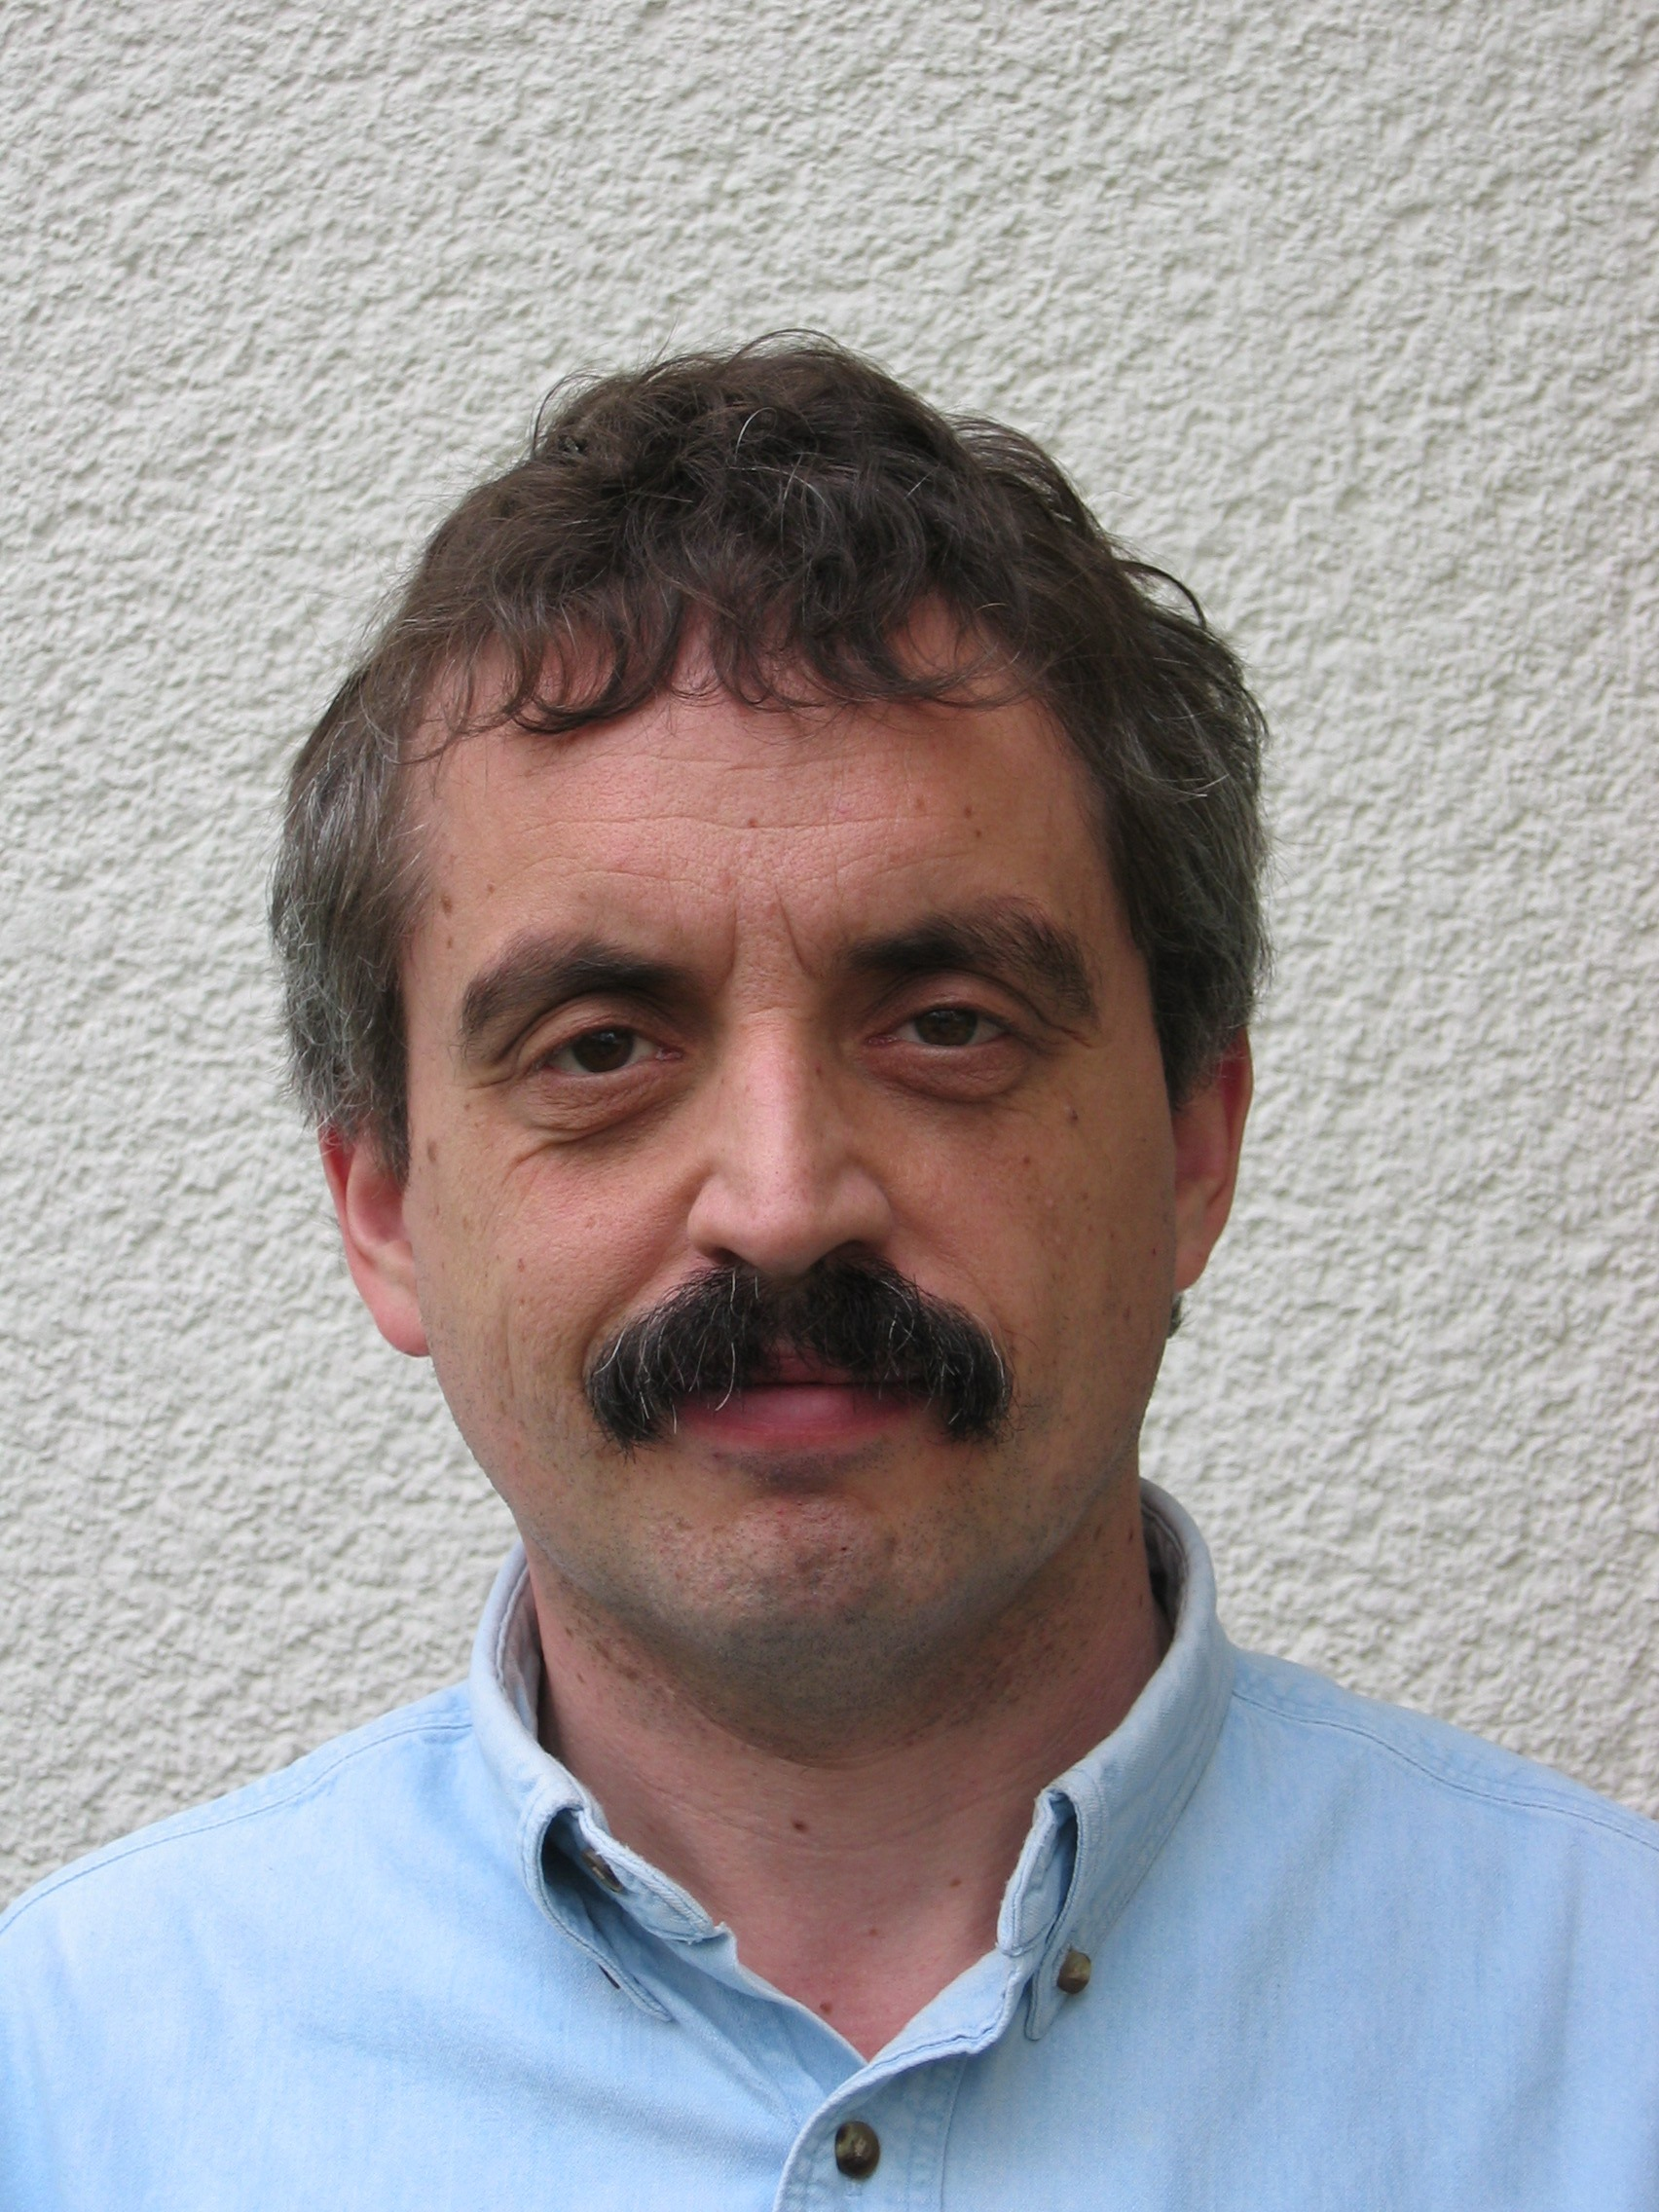
\includegraphics[width=\columnwidth, height=0.35\textheight]{res/vorstellungsfotos/wend_werner.jpg}\\
\smallskip
	Apl.\ Prof.\ Dr.\ Wend Werner\\
	Mathematisches Institut
\end{center}

Mir werden Sie in der nächsten Zeit in den Vorlesungen zur "Mathematik für Physiker" begegnen.
Mein Studium von Mathematik und Physik habe ich an der Freien Universität Berlin absolviert; Diplom und Promotion habe ich auch jeweils dort abgeschlossen.
Meine Habilitation habe ich an der Universität Paderborn gemacht und bin nun seit gut einem Jahrzehnt Hochschullehrer in Münster.

\[
	\resizebox{0.4\columnwidth}{!}{
		$\displaystyle\sum_{n = 1}^\infty \frac{1}{n^2} = \frac{\pi^2}{6}$
	}
\]

Die Themen von Promotion und Habilitation betrafen geometrische Fragen in Räumen unendlicher Dimension.
In letzter Zeit war das vor allem "Nichtkommutative Geometrie", ein Gebiet, welches versucht, einen mathematischen Formalismus zu finden, der in der Lage ist, Quanten- und relativistische Physik in einheitlicher Weise zu beschreiben.
Wie so oft beim Zusammenspiel von Mathematik und Physik sind auch hier interessante, rein mathematische Fragestellungen in Erscheinung getreten.

%\begin{center}
%	\includegraphics[width=\columnwidth, height=0.17\textheight]{private/res/comics/calvin_mathe.pdf}
%\end{center}

Der Zyklus "Mathematik für Physiker" ist eine kleine Herausforderung, da in vergleichsweise kurzer Zeit eine größere Stoffmenge vermittelt werden muss, die nichtsdestotrotz von den Teilnehmern anschließend handwerklich beherrscht werden muss.

Aber, keine Angst: Wir werden sehr langsam beginnen und erst im Laufe der Zeit Fahrt aufnehmen.
\end{multicols}

\begin{center}
	\fibelimgtext{
		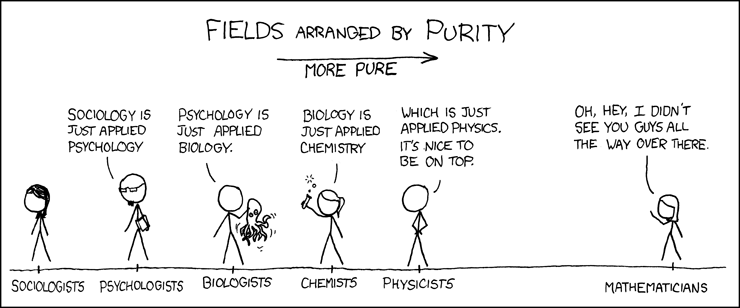
\includegraphics[width=0.9\textwidth]{res/xkcd/435_purity.png}
	}{\url{https://xkcd.com/435}}
\end{center}

\begin{multicols}{2}
\begin{center}
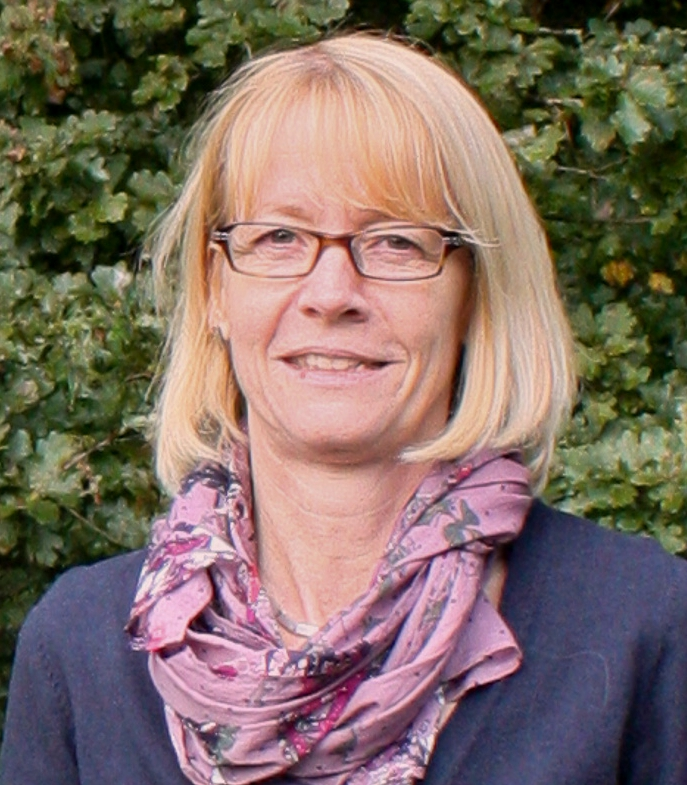
\includegraphics[width=0.8\columnwidth]{res/vorstellungsfotos/denz.jpg}\\
\smallskip
Prof.\ Dr.\ Cornelia\ Denz\\
Institut für Angewandte Physik
\end{center}

\begin{footnotesize}

Herzlich willkommen am Fachbereich Physik! Nach einigen Semestern, in denen ich Kurse im Masterstudium und für Nebenfachstudierende gelesen habe, freue ich mich sehr, gemeinsam mit meinem Kollegen Prof. Dr. Tilmann Kuhn und dem Vorlesungsteam Ihnen in den nächsten drei Semestern die Grundlagen der Physik näher zu bringen. Ich hoffe, Sie mit spannenden Experimenten und interaktiven Einheiten für die Experimentalphysik begeistern zu können. Neben den Grundlagen werden wir auch immer wieder aktuelle physikalische Entwicklungen und Highlights aus der Forschung besprechen.\\
Da der Beginn eines Studiums nicht leicht ist, werden Sie auch Methoden zum effektiven Lernen kennenlernen und Tipps zur Gestaltung des Studiums mit Auslandsaufenthalten, Industriepraktika oder ersten Forschungsprojekten erhalten.
\\[1.5ex]
Meine Arbeitsgruppe „Nichtlineare Photonik“ am Institut für Angewandte Physik beschäftigt sich mit der Strukturierung von Licht mit ultrakurzen und kohärenten Laserstrahlen. Dadurch können wir mit Licht neuartige Materialien herstellen, die besondere, bisher unbekannte Eigenschaften aufweisen. Ein Beispiel sind nanostrukturierte diskrete Materialien, die Lichteffekte der Natur nachbilden oder neue Licht-Materie Wechselwirkungen erzeugen. Ein weiteres Beispiel sind die holographische Datenspeicherung oder die quanten-optische Bildverarbeitung, die wir durch strukturiertes Licht zu höheren Kapazitäten und schnelleren Datenraten treiben. Strukturiertes Licht ermöglicht es uns auch, sogenannte holographische optische Pinzetten herzustellen, die Nanopartikel oder Zellen halten, bewegen und damit kontrollieren. Gerade die Untersuchung von Zellelastizitäten und Zellkrankheiten mit solchen optischen Pinzetten ist derzeit ein ganz aktuelles Gebiet der biomedizinischen Forschung.
\\[1.5ex]
Unser Fernziel ist es, mit strukturiertem Licht neue Anwendungen in der Biophysik, der Nanophysik und in der optischen Informationsverarbeitung zu entwickeln.
\\[1.5ex]
Unsere Forschungsthemen entwickeln wir gemeinsam in Verbünden mit Kolleginnen und Kollegen aus der Physik, Chemie, Biologie und Medizin an der Universität Münster sowie mit internationalen Partnern in vielen Ländern in Europa, aber auch in USA, Kanada, Australien und Südafrika. Wenn Sie Spaß am Experimentieren mit Licht und Lasern haben, und gerne in internationalen Teams arbeiten, sind sie bei uns genau richtig. Wir bieten auch für „junge“ Studierende die Möglichkeit, im Labor mitzuarbeiten – ob als studentische Hilfskräfte oder als studentische Forscher/-innen. So können Sie ausprobieren, ob Sie sich für eine Bachelor- oder Masterarbeit in diesem Themenbereich begeistern können.
\\[1.5ex]
Unsere Arbeitsgruppe betreibt auch das Schülerlabor MExLab („Münster’s Experimentierlabor“) Physik sowie eine Zentrum für MINT Programme für Schülerinnen und Schüler, MExLab ExperiMINTe. Im Sommer führen wir auch das Sommer-Experimentiercamp Q.UNI durch.
\\[1.5ex]
Mein Weg in die Physik begann an der Technischen Universität (TU) Darmstadt, wo ich von 1982 bis 1988 Physik studierte, aber auch Kurse in Geologie, Soziologie und Philosophie belegte. Da mir die interdisziplinäre Arbeitsweise der Optik gefiel, habe ich meine Diplomarbeit über ein Thema der Lichtverstärkung durch nichtlineare optische Materialien geschrieben und dabei mit einer Gruppe aus Frankreich kooperiert. Ein Teil meiner Promotion habe ich danach am Institut d’Optique in Orsay bei Paris in Frankreich verbracht und dabei an optischer Datenspeicherung geforscht. Nach meiner Promotion wurde ich wissenschaftliche Assistentin am Institut für Angewandte Physik der TU Darmstadt, und forschte im Bereich der Strukturbildung in nichtlinearen optischen Systemen, einem interdisziplinären Thema der nichtlinearen Physik. Daher habe ich seit meiner Berufung an die WWU 2001 in den Forschungsschwerpunkten Nichtlineare Physik und Nanophysik engagiert und gemeinsam mit einigen Kollegen das Center for Nonlinear Science gegründet.
\\[1.5ex]
Mir ist die Partizipation aller an der Physik sehr wichtig, denn nur durch internationale und diverse, vielfältige Teams können wir heute die Forschung mit neuen Ideen voranbringen. Daher habe ich seit 2016 neben meiner Professur für Angewandte Physik auch eine Professur für Geschlechterforschung in der Physik inne. Ziel dieser Arbeitsgruppe ist die Analyse und Verbesserung der Situation von Frauen in der Physik, sowie die Etablierung der Geschlechterforschung im Sinne von Wissenschaftsforschung in diesem Fachgebiet. Im Zentrum steht daher die Leitfrage nach dem Verhältnis von Wissenschaft, Gesellschaft und Geschlecht in der Physik.
\\[1.5ex]
Im integrierten Kurs möchte ich auch versuchen, Ihnen die interdisziplinären, internationalen und vielfältigen Aspekte der Physik näher zu bringen, Sie für einen offenen, neugierigen Blick auf die Physik in Ihrer Umgebung zu interessieren und Sie bei den ersten Schritten im Physikstudium zu unterstützen.
\\[1.5ex]
Ich wünsche Ihnen damit einen erfolgreichen Start und viel Freude beim Studium der Physik.

\end{footnotesize}
\end{multicols}

\newpage

\begin{multicols}{2}
\begin{center}
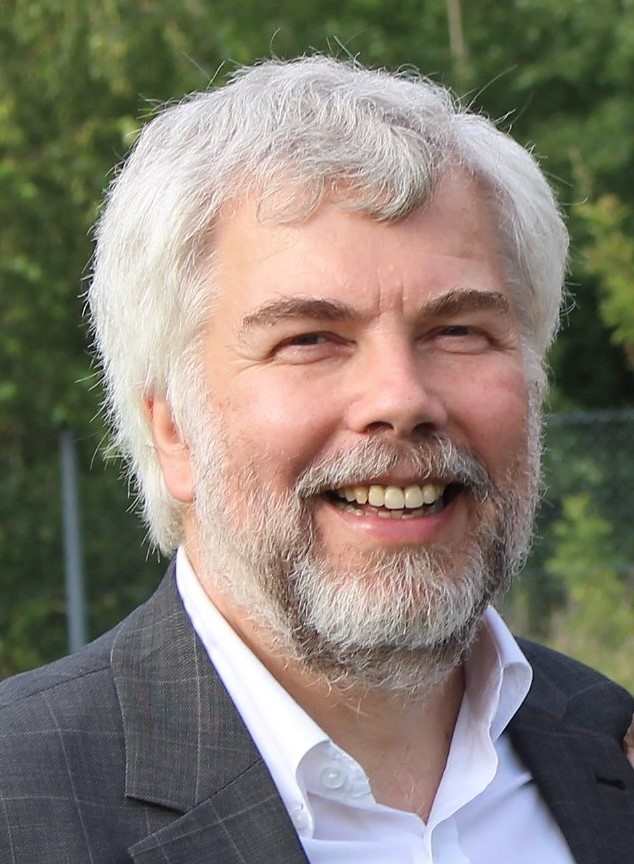
\includegraphics[width=0.71\columnwidth]{res/vorstellungsfotos/kuhn.jpg}\\
\smallskip
Prof.\ Dr.\ Tilmann Kuhn\\
Institut für Festkörpertheorie
\end{center}

Seit dem Sommersemester 1996 bin ich Professor am Institut für Festkörpertheorie der Westfälischen Wilhelms-Universität Münster. Wie schon der Name des Instituts nahelegt, sind meine Forschungsaktivitäten im Bereich der theoretischen Festkörperphysik angesiedelt. Hier interessieren mich speziell ultraschnelle dynamische Prozesse in Festkörpern und Nanostrukturen, die eine wichtige Rolle für das Verständnis der optischen und elektronischen Eigenschaften dieser Materialien spielen. In der Lehre habe ich in den 22 Jahren, die ich jetzt in Münster tätig bin, neben verschiedenen Wahlpflicht- und Spezialvorlesungen auch mehrfach alle Kursvorlesungen der theoretischen Physik im Bachelorstudiengang gelesen. Seit etwas mehr als zwei Jahren bin ich darüber hinaus Studiendekan des Fachbereichs Physik und damit für den Bereich Studium und Lehre im Fachbereich zuständig.

Nachdem ich in den vergangenen Semestern überwiegend Lehrveranstaltungen im Masterstudiengang gehalten habe, freue ich mich, in den kommenden drei Semestern mal wieder den theoretischen Teil des Kurses Physik I-III zu lesen. Gemeinsam mit meiner Kollegin Prof. Dr. Cornelia Denz möchte ich Ihnen den für die Physik typischen Zugang zum Verständnis der Naturgesetze nahebringen, der aus einer Kombination von experimenteller Beobachtung und theoretischer Beschreibung besteht. Speziell im Theorieteil wird es in den nächsten drei Semestern darum gehen, zum einen grundlegende mathematische Techniken bereit zu stellen, die im Verlauf des Studiums immer wieder benötigt werden, und zum anderen einen ersten Einblick in die Denk- und Arbeitsweise der theoretischen Physik anhand der Gebiete Mechanik, Thermodynamik, Elektrodynamik, Optik und Relativitätstheorie zu vermitteln.

Vor genau 40 Jahren, im Herbst 1978, begann mein Weg in die Physik mit der Aufnahme des Physikstudiums an der Universität Stuttgart. Dort habe ich 1987 auch promoviert. Von 1989 bis 1991 war ich dann für zwei Jahre mit einem Stipendium der Deutschen Forschungsgemeinschaft als Postdoktorand an der Università degli Studi di Modena in Italien. Neben einer sehr fruchtbaren wissenschaftlichen Tätigkeit mit den Kolleginnen und Kollegen der dortigen Arbeitsgruppe hat mir dieser Auslandsaufenthalt auch viele wichtige Erfahrungen und Eindrücke vom Leben in einem anderen Land vermittelt, die ich nicht missen möchte. Anschließend kehrte ich nach Stuttgart zurück, wo ich mich im Jahr 1994 habilitierte und auch meine ersten Doktoranden betreute. Vom Herbst 1994 bis zum Frühjahr 1996 hatte ich eine Vertretungsprofessur für Theoretische Physik an der Brandenburgischen Technischen Universität Cottbus, wo ich am Aufbau des dortigen Physik-Studiengangs mitwirken konnte. Während dieser Zeit erhielt ich den Ruf auf eine Professur für Theoretische Physik an der Universität Münster, den ich gerne annahm, so dass ich seit April 1996 in diesem Fachbereich in Lehre und Forschung tätig bin.

In der Forschung beschäftige ich mich zusammen mit den Bachelor- und Masterstudierenden sowie den Doktoranden und Postdoktoranden meiner Arbeitsgruppe mit der theoretischen Modellierung dynamischer Prozesse in Systemen wie magnetischen Schichten, Supraleitern, ultrakalten Fermigasen und Halbleitern. Einen Schwerpunkt bildet dabei die ultraschnelle Dynamik in modernen Halbleiter-Nanostrukturen, insbesondere nach Anregung mit Femtosekunden-Laserpulsen (1\,fs = $10^{-15}$\,s). Dies ist die charakteristische Zeitskala, auf der viele elementare Wechselwirkungsprozesse ablaufen, deshalb kann man durch solche Untersuchungen viel über die Natur der grundlegenden Wechselwirkungsmechanismen in Festkörpern lernen. Außerdem ist die Dynamik hier häufig von charakteristischen Quantenphänomenen geprägt, wie etwa dem Auftreten verschränkter Zustände oder kohärenter Überlagerungszustände, die für mögliche Anwendungen im Bereich der Quanteninformationsverarbeitung und der Quantenkryptographie von zentraler Bedeutung sind.

\end{multicols}
